We developed a semi-structured interview protocol to explore how educators
across a variety of tertiary insitutions. In
Section~\ref{subsec:interview-questions}, we describe the interview questions
that we developed and in Subsection~\ref{subsec:interview-probes} we describe
the taxonomy of interview probes we empoloyed to guide consistent follow-up
questions across interviews. Following this, in
Section~\ref{sec:data-collection} we describe our recruitment and data
collection procedures. Finally, in Section~\ref{sec:data-analysis} we describe
our approach to analyzing the data collected through these interviews.

\begin{figure*}[ht]
  \centering
  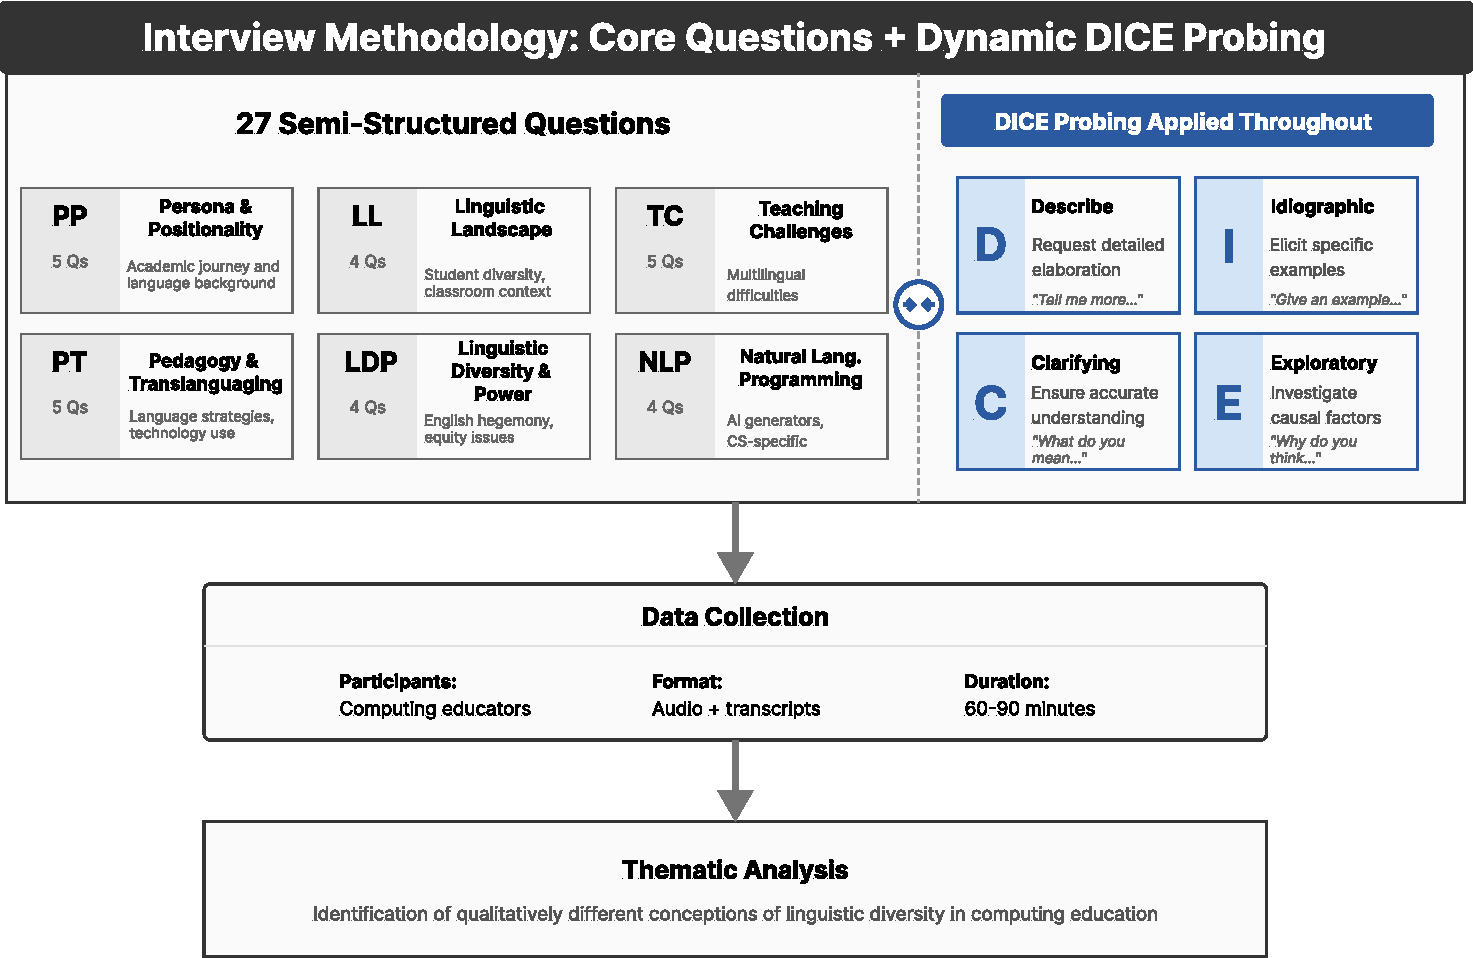
\includegraphics[width=\textwidth]{imgs/methods.pdf}
  \caption{Your caption here.}
  \label{fig:methods}
\end{figure*}


\subsection{Interview Questions}\label{subsec:interview-questionse

\subsubsection{Persona and Positionality}\label{subsubsec:persona-and-positionality}

% Context and grounding
Given the phenomenographic nature of this work, it is important that we
understand the context and positionality of each participant. These questions
are designed to provide this context---with particular focus on the
educational, instructional, and linguistic backgrounds of each participant. The
questions, in this regard, are as follows:
\begin{enumerate}[label={PP.\arabic*}, align=left, leftmargin=4em]
  \item Could you briefly describe your academic journey and how you came to
    teach in your current position?
  \item What subjects do you currently teach, what levels (e.g., undergraduate,
    graduate) are these courses, and in what contexts (e.g., in-person, online,
    hybrid) are they delivered?
  \item What languages do you speak, and in what contexts do you typically use
    each?
  \item In your own education, what language(s) were used for instruction?
  \item What are your general thoughts and beliefs about the role of language in
    education, particularly in technical fields like computer science?
\end{enumerate}
Probes during this section of the interview focused on understanding
\textcolor{red}{TBD}.

\subsubsection{Linguistic Landscape}\label{subsubsec:linguistic-landscape}

Related to understanding the persona of each participant, it is essential to
underastand the linguistic landscape in which they operate. This includes not
only the languages spoken by their students, but also the languages used in
instruction
\begin{enumerate}[label={LL.\arabic*}, align=left, leftmargin=4em]
  \item How would you describe the linguistic diversity of your current students? 
  \item Your second question here
\end{enumerate}

\subsubsection{Teaching Challenges}\label{subsubsec:teaching-challenges}

\begin{enumerate}[label={TC.\arabic*}, align=left, leftmargin=4em]
  \item What are the biggest challenges you face teaching topics in
    computing to students who speak a variety of languages?
  \item Can you describe 
\end{enumerate}

\subsubsection{Pedagogy and Translanguaging}\label{subsubsec:pedagogy-and-translanguaging}

In this section, we explore the intersection of translanguaging practices and
pedagogical strategies employed by educators in multilingual settings.
\textcolor{red}{<Resaerch on india specifically and findings that inform these
questions>}.The questions are designed to uncover how educators navigate---or
leverage---the linguistic diversity of their classrooms.
\begin{enumerate}[label={PT.\arabic*}, align=left, leftmargin=4em]
  \item How do you decide when to use a particular language for
    instruction or explanation during your classes and when, if at all, do
    to change languages?
  \item If you've adopted a teaching strategy that helps you navigate
    linguistic diversity, can you describe it and why you find it effective?
  \item How do you use technology, if at all, to support students with
    different language backgrounds?
\end{enumerate}

\subsubsection{Linguistic Diversity and Power}\label{subsubsec:linguistic-diversity-and-power}

Central to language is the notion of power. The use of language carries with it
implications of power, privilege, and access. As noted by \citet{jhingran2009hundreds},
\begin{quote}
  ``\textit{English is seen as the language of power and the vehicle for getting better jobs. Even poor families in urban areas aspire to send their children to these private English-medium schools.}''
\end{quote}
Similarly, as noted by \citet{mohanty2017language}, beyond the 22 scheduled
languages, there are little instruction at the primary and secondary levels of
education which creates a systemic hierarchy of language: English and Hindi at
the top, regional scheduled languages in the middle, and minority and tribal
languages at the bottom. In this section, we explore how educators in computing
education perceptions and experiences with the role of power and privilege in
the context of linguistic diversity. 
\begin{enumerate}[label={LDP.\arabic*}, align=left, leftmargin=4em]
  \item How do you perceive the role of English in your institution and
    field of study?
  \item Have you observed any instances where language has influenced
    students' academic performance or participation in class? Can you describe
    one such instance?
  \item How do you address issues of linguistic equity in your classroom?
  \item What are your thoughts on the use of local languages versus
    English in higher education, particularly in technical fields like computer
    science?
\end{enumerate}

\subsubsection{Natural Language Programming}\label{subsubsec:natural-language-programming}

This section explores the perceptions and experiences of educators regarding
the use of natural language programming tools, such as AI-driven code
generators, in multilingual educational settings. The questions aim to uncover
how these tools are integrated into teaching practices and their impact on
students with diverse linguistic backgrounds.
\begin{enumerate}[label={NLP.\arabic*}, align=left, leftmargin=4em]
  \item What concerns or difficulties have you encountered with respect
    to linguistic diversity that you feel are specific to teaching topics in computing?
  \item Have you integrated or do you have plans to integrate any
    natural language programming tools (e.g., AI code generators) into your
    teaching? 
\end{enumerate}


\subsection{Interview Probes}\label{subsec:interview-probes}
In conducting these interviews we use probes aligned with the DICE
(\textit{``Describe, Idiographic, Clarifying, Exploratory''}) taxonomy as
described in \citet{robinson2023probing}. In more detail, the four types of
probes are:
\begin{enumerate}
  \item \textbf{Describe Probe:} These probes ask that participants provide more
    detail about a specific situation or experience they mentioned. These probes
    often take the form of \textit{``Tell me more about...''} or \textit{``Do
    you recall what was happening when...''}.
  \item \textbf{Idiographic Probe:} These probes encourage participants to share
    a specific example from a specific period of time. These probes often take
    the form of \textit{``Can you give me an example of...''} or \textit{``Do
    you recall what was happening the week you...''}.
  \item \textbf{Clarifying Probe:} These probes are used to ensure that the interviewer
    accurately understands what the participant is saying. These probes often
    take the form of \textit{``What do you mean by...''} or \textit{``Can you
    expand on...''}.
  \item \textbf{Exploratory Probe:} These probes encourage participants to think
    about the causal factors or underlying reasons behind their thoughts,
    opinions and experiences. Such questions take the form of \textit{``Why do
    you that happened?''} or \textit{``What do you think led to...''}.
\end{enumerate}
This taxonomy is designed to help interviewers structure follow-up questions in
a way that encourages participants to provide rich, detailed responses. 



\subsection{Data Collection}\label{sec:data-collection}



\subsection{Data Analysis}\label{sec:data-analysis}
